\section{Processi primari}
    \subsection{Fornitura}
    	In questo paragrafo vengono documentate le norme che i membri devono seguire affinché il gruppo possa diventare committente dei professori Vardanega e Cardin ed essere fornitori dell'azienda Zucchetti\pedice.
    \subsubsection{Studio di fattibilità}
        Dopo la presentazione dei capitolati il gruppo si è riunito per discutere la scelta più consona. Dopo aver risolto i dubbi interni ed aver redatto lo studio di fattibilità, documento, ad oggi \textit{in versione 1.0.0},  atto a valutare i pro e i contro di ogni progetto permettendo così una più attenta valutazione, si è optato per la scelta del capitolato \textit{numero 3}.  \newline
        I punti chiave dell'analisi sono i seguenti:
    	\begin{itemize}
		   \item \textbf{Introduzione:} Viene fatta una breve introduzione del contesto in cui applicare la soluzione;
		   \item \textbf{Finalità:} Viene descritto in modo sintetico lo scopo finale da raggiungere a lavoro completato;
		   \item \textbf{Tecnologie in uso:} Si descrivono genericamente i software che la proponente intende usare;
		   \item \textbf{Conclusioni:} Rappresenta il motivo per cui un capitolato è stato scelto oppure scartato.
	    \end{itemize}
	    Per  discutere  in  dettaglio  i  requisiti  richiesti  dalla  proponente  e  poter  arrivare ad un accordo finale che sancisca il contratto a cui le due parti devono attenersi e rispettare,  il gruppo Dream Corp. si impegna a mantenere un colloquio costante e uno spirito di collaborazione al fine di agevolare entrambe le parti per la miglior riuscita del prodotto.  Questo permetterà un continuo colloquio al fine di far fronte:
	    \begin{itemize}
	        \item A determinati bisogni da parte della proponente, per soddisfare, se possibile, le richieste avanzate;
	        \item Alla determinazione dei vincoli sul prodotto;
	        \item Alla determinazione della qualità che il prodotto dovrà perseguire.
	    \end{itemize}
	    A seguito della consegna del prodotto, il gruppo Dream Corp., salvo diversi accordi con la proponente Zucchetti, non intraprenderà attività di manutenzione del prodotto.
	    
    \subsubsection{Documentazione fornita}
	    Al fine di assicurare massima trasparenza e qualità alla proponente ed ai committenti verranno elencati i documenti forniti con una breve descrizione del loro contenuto:
    	\begin{itemize}
	        \item \textbf{Piano di progetto:} descrive la pianificazione, la consegna e il suo completamento;
	        \item \textbf{Analisi dei requisiti:} viene definita l'analisi dei casi d'uso e dei requisiti del gruppo
	        \item \textbf{Piano di qualifica:} verifica, validazione e garanzia della qualità dei processi e di prodotto.
	    \end{itemize}
    \newpage    
\subsection{Sviluppo}
    \subsubsection{Analisi dei requisiti}
    	L'Analisi dei Requisiti viene scritta dagli Analisti che hanno il compito di valutare in modo accurato ogni aspetto del progetto. In particolare, questo documento è redatto con lo scopo di:
	    \begin{itemize}
	    	\item Descrivere scopo e funzionalità del prodotto;
	    	\item Fornire i requisiti e vincoli concordati col cliente;
	    	\item Descrivere gli elementi principali che hanno un ruolo chiave nello sviluppo del prodotto;
	    	\item Definire tutti i casi d'uso;
	    	\item Tracciare in modo dettagliato tutti i requisiti.\newline
	    \end{itemize}
    	L'Analisi dei Requisiti seguirà le specifiche descritte in seguito.\newline \newline
    	\textbf{Classificazione casi d'uso}  Al fine di classificare e rendere leggibili i casi d'uso abbiamo deciso di utilizzare una codifica per descriverli. Ad ogni caso d'uso verrà quindi associata una stringa univoca strutturata nel seguente modo:
        \begin{equation}
            UCX.Y.Z    
        \end{equation}
        dove X,Y,Z sono dei numeri progressivi per indicare specificità all'interno dei casi d'uso. \newline
        \newline
        Per rappresentare una scelta tra casi d'uso tra loro mutuamente esclusivi abbiamo deciso di adottare il seguente criterio: nella codifica del caso d'uso verrà aggiunta una lettera maiuscola, tra parentesi tonde, per indicare un insieme di scelte per risolvere il caso d'uso generico, rappresentato dalla normale codifica numerica X.Y.Z. La finale codifica di un caso d'uso di specializzazione sarà quindi:
        \begin{equation}
            UCX(A).Y(A).Z(A)
        \end{equation}
        L'utilizzo di tale criterio sarà utilizzato solo in caso di bisogno e quindi non è detto che sia presente in tutti i casi d'uso.\newline
	    Ogni caso d'uso è inoltre definito secondo la seguente struttura:\newline
	    \begin{itemize}
	    	\item \textbf{ID:} il codice del caso d'uso secondo la convenzione specificata poco sopra;
	    	\item \textbf{Nome:} titolo del caso d'uso;
	    	\item \textbf{Descrizione:} breve descrizione del caso d'uso;
	    	\item \textbf{Precondizione:} condizioni assunte come vere prima del verificarsi degli eventi del caso d'uso;
	    	\item \textbf{Postcondizione:} condizioni assunte come vere dopo il verificarsi degli eventi del caso d'uso;
	    	\item \textbf{Attori:} attori principali e secondari (se presenti) del caso d'uso;
	    	\item \textbf{Scenario Principale:} flusso degli eventi rappresentato attraverso una lista numerata.\newline
	    \end{itemize}
	    Nella \textit{Figura 1} viene riportato un esempio di caso d'uso:\newline
    
	    \begin{figure}[!htbp]
	    	\centering
	    	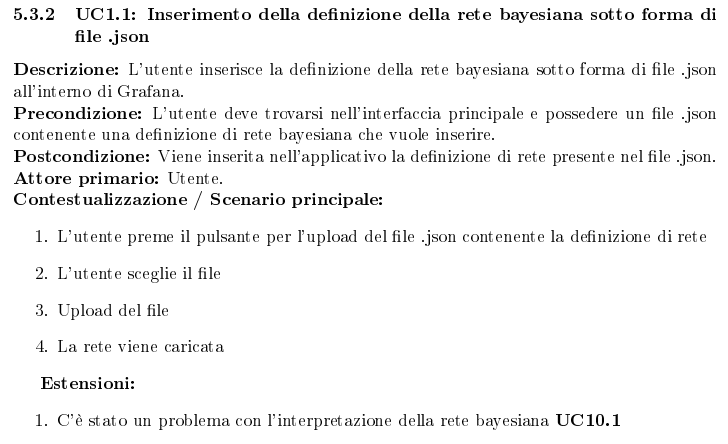
\includegraphics[scale=0.7]{casoduso.png}
	    	\caption{Esempio di caso d'uso}
	    \end{figure}
    
	    ~\newline \textbf{Classificazione dei requisiti} Tutti i requisiti ottenuti dopo una profonda analisi degli Analisti possono essere ricavati da tre diverse fonti:\newline
	    \begin{itemize}
	    	\item \textbf{Interno:} il requisito proviene da una decisione del gruppo Dream Corp., generalmente emersa durante un incontro e riportata in un verbale;
	    	\item \textbf{Capitolato:} il requisito proviene dalle richieste del capitolato;
	    	\item \textbf{Esterno:} il requisito proviene da un incontro con la proponente.\newline
	    \end{itemize}
	    Il codice utilizzato per indicizzare univocamente i requisiti è il seguente:\newline
	    \begin{center}
	    	\textbf{R+(F|Q|V|P)+(C|O)+(X(.Y)*)}
	    \end{center}
	    \begin{itemize}
	    	\item \textbf{R:} Requisito;
	    	\item \textbf{F|Q|V|P:}
	    	\begin{itemize}
	    		\item F: Requisito funzionale che descrive nel dettaglio i servizi che verranno forniti dal sistema agli attori;
	    		\item Q: Requisito di qualità;
	    		\item V: Requisito di vincolo;
	    		\item P: Requisito prestazionale;
	    	\end{itemize}
	    	\item \textbf{C|O:}
	    	\begin{itemize}
	    		\item C: Compulsory (obbligatorio);
	    		\item O: Optional (opzionale);
	    	\end{itemize}
	    	\item \textbf{X.Y:} Numeri naturali concatenati con un punto per descrivere un sottorequisito.\newline
	    \end{itemize}
	    I requisiti di vincolo, di qualità e prestazionali fanno parte dei requisiti non funzionali che descrivono i vincoli sul sistema e sul suo processo di sviluppo.
	    Ad ogni requisito verranno infine associate la sua priorità, una breve descrizione e le sue fonti come nella \textit{Figura 2}.\newline
	    
	    \begin{figure}[!htbp]
	    	\centering
	    	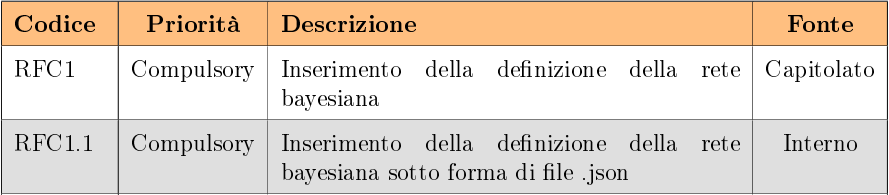
\includegraphics[scale=0.45]{requisiti.png}
	    	\caption{Esempio di requisito}
	    \end{figure}
	    
	    ~\newline\textbf{Tracciamento} Infine, per facilitare la lettura e la visualizzazione dei requisiti, questi verranno indicizzati in due modalità specifiche:
	    \begin{itemize}
	    	\item \textbf{Tracciamento Priorità-Requisito:} il focus è orientato sulla priorità;
	    	\item \textbf{Tracciamento Tipologia-Requisito:} il focus è orientato sulla tipologia.\newline
	    \end{itemize}
	    Per una lettura immediata non sono riportate le descrizioni per le quali si rimanda alle sezioni apposite nel documento \AdR.
	    Infine, viene riportata una tabella riassuntiva che permette di avere un quadro generale della distribuzione dei requisiti.\newline

	    \subsubsection{Progettazione}
	    \paragraph{Scopo}~\newline ~\newline
	    L'attività di Progettazione consiste nel descrivere una soluzione al problema che sia soddisfacente per tutti gli stakeholders\pedice.~Ciò serve a garantire che il prodotto sviluppato soddisfi le qualità, le proprietà e i bisogni nell'attività di analisi. L'architettura definita, secondo le metriche descritte in appendice sezione \textit{\underline{C.2}}, dovrà avere le seguenti qualità:
	    \begin{itemize}
	        \item \textbf{Sufficienza} deve soddisfare i requisiti definiti nel documento \textit{Analisi dei requisiti};
	        \item \textbf{Comprensibilità} affinché possa essere capita dagli stakeholder;
	        \item \textbf{Flessibilità} deve  poter  permettere  modifiche  al  variare  o  all’aggiunta  di requisiti senza perdite di performance o doverla restaurare profondamente;
	        \item \textbf{Affidabilità} deve avere una elevata capacità di rispettare le specifiche nel tempo;
	        \item \textbf{Sicurezza} rispetto ad intrusioni e malfunzionamenti;
	        \item \textbf{Incapsulazione} le componenti dovranno essere progettate in modo che le informazioni interne siano nascoste;
	        \item \textbf{Coesione} in modo che le parti che hanno gli stessi obiettivi stanno insieme;
	        \item \textbf{Basso accoppiamento} parti distinte devono essere poco dipendenti l’una dalle altre, in modo da poter essere facilmente mantenibili.
	    \end{itemize}
	    
	    \paragraph{Obiettivi della progettazione}~\newline ~\newline
	    Essa serve a garantire che il prodotto sviluppato soddisfi le proprietà e i bisogni specificati nell'attività di analisi ponendo i seguenti obiettivi:
	    \begin{itemize}
    	    \item Garantire la qualità di prodotto sviluppato, perseguendo la correttezza per costruzione;
            \item Organizzare e ripartire compiti implementativi, riducendo la complessità del problema originale fino alle singole componenti facilitandone la codifica da parte dei singoli Programmatori;
            \item Rendere chiara e comprensibile ogni parte dell'architettura ai differenti stakeholders;
            \item Mantenere nascosti i dettagli implementativi, seguendo il principio dell'information hiding;
            \item Mantenere bassa la dipendenza tra le varie parti del prodotto, seguendo il principio della modularità;
            \item Ottimizzare l’uso di risorse.
        \end{itemize}
	    
	    \paragraph{Diagrammi}~\newline
	    Al fine di essere il più comprensibili possibile sarà necessario far uso su larga scala di diagrammi UML\pedice 2.0, utilizzando le seguenti rappresentazioni:
	    \begin{itemize}
	        \item \textbf{Diagrammi dei casi d'uso:}
	        \item \textbf{Diagrammi delle classi:}
	        \item \textbf{Diagrammi di attività:}
	    \end{itemize}
	    Per poter rappresentare i diagrammi secondo rappresentazioni appena descritti verrà utilizzato PlantUML\footnote{\url{http://plantuml.com}}.
	    
	    \paragraph{Diagrammi delle classi}
	    Lo scopo dei diagrammi delle classi può essere sintetizzato in:
	    \begin{itemize}
	        \item Analisi e progettazione della visione statica di un’applicazione;
             \item Descrizione delle responsabilità di un sistema;
	    \end{itemize}
	    Per stabilire le relazioni tra le classi e avere una rappresentazione totale del prodotto verrà creato un file con estensione \textbf{.puml} successivamente verrà inclusa ogni classe con estensione \textbf{.iuml} con la comodità di avere ogni cambiamento applicato alla singola classe riflesso nella struttura finale.\\
	    I diagrammi delle classi sono collegati fra loro da frecce che esplicitano le dipendenze. In particolare, verranno utilizzati i seguenti tipi di freccia:
	    \begin{itemize}
	        \item Freccia semplice, dalla classe A alla classe B: indica che la classe A ha fra i propri campi dati una o più istanze della classe B;\par
    	    \begin{minipage}{\linewidth}
        		\centering
        		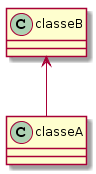
\includegraphics{dipendenzaForteTraAeB.png}
    	        \captionof{figure}{Esempio di dipendenza forte tra classi}
        	\end{minipage}
        	\item Freccia tratteggiata, dalla classe A alla classe B: indica una dipendenza, significa che A dipende da B secondo una primitiva che dovrà essere esplicitata vicino alla freccia;\par
    	    \begin{minipage}{\linewidth}
        		\centering
        		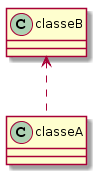
\includegraphics{dipendenzaDeboleTraAeB.png}
        		 \captionof{figure}{Esempio di dipendenza debole tra classi}
        	\end{minipage}
        	\item Freccia a diamante vuota, dalla classe A alla classe B: indica un’aggregazione, una relazione non forte ovvero una relazione nella quale le classi parte hanno un significato anche senza che sia presente la classe tutto;\par
        	\begin{minipage}{\linewidth}
        		\centering
        		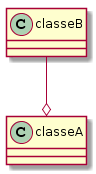
\includegraphics{aggregazioneTraAeB.png}
        		 \captionof{figure}{Esempio di aggregazione tra classi}
        	\end{minipage}
        	\item Freccia a diamante piena, dalla classe A alla classe B: indica la composizione, definita come una relazione forte cioè una relazione nella quale le classi parte hanno un reale significato solo se sono legate alla classe tutto;\par
        	 \begin{minipage}{\linewidth}
        		\centering
        		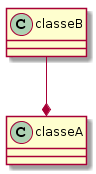
\includegraphics{composizioneTraAeB.png}
        		 \captionof{figure}{Esempio di composizione tra classi}
        	\end{minipage}
        	\item Freccia vuota, dalla classe A alla classe B: indica l’ereditarietà/generalizzazione ed è il massimo grado di dipendenza fra classi. Indica che ogni oggetto di A è anche un oggetto di B.\par
        	 \begin{minipage}{\linewidth}
        		\centering
        		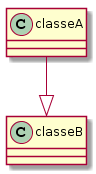
\includegraphics{ereditarietaTraAeB.png}
        		 \captionof{figure}{Esempio di ereditarietà tra classi}
        	\end{minipage}
	    \end{itemize}
	    
	    \paragraph{Diagrammi di attività}~\newline ~\newline
	    I diagrammi delle attività conterranno i seguenti elementi collegati sempre da frecce, che verranno indicati con i formalismi indicati:
	    \begin{itemize}
	        \item Nodo iniziale, rappresentato da un pallino pieno. È il punto da cui inizia l’esecuzione. Genera un token;
            \item Activity, rappresentata da un rettangolo che ne contiene la descrizione. La descrizione dovrà essere il più breve e concisa possibile, è possibile una sin- tassi sincopata della frase, composta per lo più da parole chiave. Consuma e produce un token;
            \begin{figure}[!htbp]
    		    \centering
    		    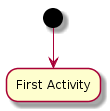
\includegraphics{firstActivity.png}
    		    \captionof{figure}{Esempio del nodo iniziale del diagramma attività}
	        \end{figure}
	        \item Subactivity, rappresentata da un rettangolo che ne contiene il nome (sempre indicato con la lettera maiuscola) e un piccolo tridente nell'angolo in basso a destra. è un riferimento ad una il cui diagramma viene descritto separatamente. Ogni sotto attività ha un input ed un output;
            \item Branch, rappresentato da un rombo con una freccia in ingresso e n in uscita. è un punto in cui si può prendere solo uno degli n rami, ognuno dei quali deve avere scritta in prossimità la guardia, secondo il formato [guardia]. Consuma e produce un token;
            \item Merge, rappresentato da un rombo con n frecce in ingresso e una in uscita. è un punto in cui gli n rami generati da un Branch tornano ad unirsi. Consuma e produce un token;\par
            \begin{figure}[!htbp]
    		    \centering
    		    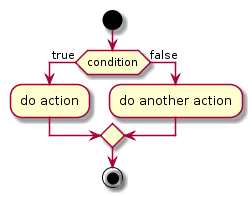
\includegraphics{branchEMerge.png}
    		    \captionof{figure}{Esempio del nodo branch e merge del diagramma attività}
            \end{figure}
            \item Fork, rappresentato da una linea lunga orizzontale o verticale. \'E un punto in cui l'attività si parallelizza senza vincoli di esecuzione temporale, ha una freccia in ingresso e N in uscita. Consuma un token e ne genera n;
            \item Join, rappresentato da una linea lunga orizzontale o verticale. è un punto in cui avviene la sincronizzazione fra processi paralleli, ha N frecce in ingresso e una in uscita. Consuma n token e ne genera uno;\par
            \begin{minipage}{\linewidth}
    		    \centering
    		    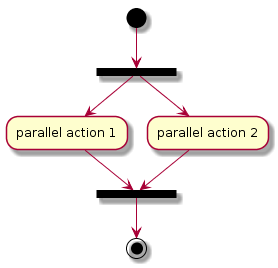
\includegraphics{forkEJoin.png}
    		    \captionof{figure}{Esempio di fork e join del diagramma attività}
            \end{minipage}
            \item Pin, rappresentato da un piccolo quadratino dove entrano/escono frecce dalle Activity. Indica il passaggio di un parametro, il cui tipo va indicato di fianco secondo il formato TipoParametro;
            \item Segnali, rappresentati da due figure a incastro, la prima (non bloccante) per l’emissione del segnale, la seconda (bloccante) per la ricezione dello stesso.\par
            \begin{minipage}{\linewidth}
        		\centering
        		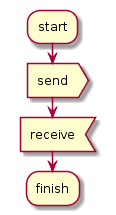
\includegraphics{sendReceive.png}
        		 \captionof{figure}{Esempio di invio e ricezione del diagramma attività}
    	    \end{minipage}
        	\item Timeout, rappresentato da una clessidra, serve per modellare timeout o eventi ripetuti. I timeout hanno frecce entranti e frecce uscenti, al contrario degli eventi ripetuti che possono avere solo archi uscenti. Di fianco devono avere una descrizione così composta: i timeout devono cominciare con "wait" e le azioni ripetute con ”every”, di seguito dovrà trovarsi un'indicazione temporale o una descrizione in linguaggio naturale breve e concisa;
        	\item Nodo di fine flusso, rappresentato da un cerchio vuoto con una X al centro. È un punto in cui uno dei rami di esecuzione va a morire, ma l’esecuzione continua comunque sugli altri rami paralleli. Consuma un token;\par
        	\begin{minipage}{\linewidth}
        		\centering
        		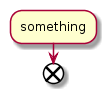
\includegraphics{fluxFinished.png}
    		    \captionof{figure}{Esempio di nodo di nodo di fine flusso del diagramma attività}
	        \end{minipage}
            \item Nodo finale, rappresentato da due cerchi concentrici di cui il più esterno vuoto e il più interno pieno. È il punto da cui termina l’esecuzione. Consuma un token.\par
            \begin{minipage}{\linewidth}
        		\centering
        		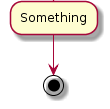
\includegraphics{finish.png}
    		    \captionof{figure}{Esempio di nodo di nodo finale del diagramma attività}
	        \end{minipage}
	    \end{itemize}
       

	    
	    \paragraph{Sviluppo}~\newline ~\newline
	    Lo sviluppo di \textit{G\&B} avviene seguendo il modello incrementale spiegato nel \PdP nella sezione \textit{\underline{3}}. Eseguiremo un’analisi comparativa di varie tecnologie esistenti al fine di capire quali siano le più consone allo sviluppo di \textit{G\&B}.  Nel caso si ritengano più consone tecnologie differenti da quelle proposte dalla proponente, il gruppo Dream Corp. si riserva di discutere con la stessa per discuterne. La proponente identifica queste tecnologie come obbligatorie per lo sviluppo:
	    \begin{itemize}
	        \item \textbf{Javascript\pedice};
	        \item \textbf{Angular};
	        \item \textbf{Node.js\pedice};
	        \item \textbf{Html}.
	    \end{itemize}
	    \paragraph{Continuous integration}~\newline ~\newline
	    L'attività di continuous integration sarà effettuata utilizzando Travis\pedice integrato con la repository del progetto. Travis crea una build ed esegue automaticamente i test di unità. In questo modo sarà possibile identificare e correggere immediatamente le modifiche. Per quanto riguarda il test coverage, cioè il grado di esecuzione del codice sorgente durante l’esecuzione dei test, verrà utilizzato il tool Jest\pedice. Infine, verrà utilizzato il servizio Coveralls\pedice per la proiezione di un "cruscotto informativo" contenenti i valori di copertura del codice.
	    \begin{figure}[!htbp]
		    \centering
		    
\includegraphics{BuildPassed.png}
		    \caption{Esempio di Build eseguita con successo da Travis}
	    \end{figure}
	    
    	\begin{figure}[!htbp]
		    \centering
		    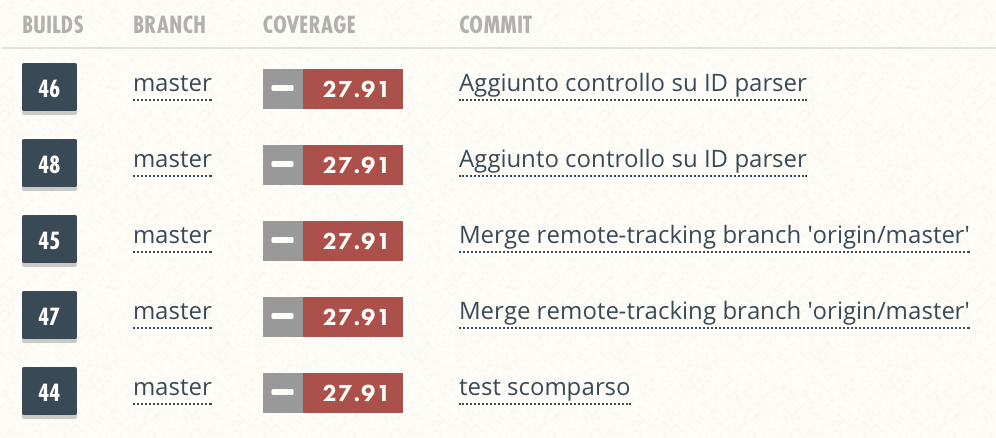
\includegraphics{CruscottoInformativoCoveralls.png}
		    \caption{Esempio di Code coverage}
	    \end{figure}
	\clearpage
	    \subsubsection{Codifica}
	In  questa  sottosezione  vengono  elencate  le  norme   alle  quali  i  Programmatori  devono attenersi durante l’attività di programmazione ed implementazione. Ogni  norma è  rappresentata  da  un  paragrafo contenente un titolo,  una breve descrizione e, se necessario, un esempio esplicativo.  Alcune di esse possono anche contenere una lista di possibili eccezioni d’uso. L’uso di norme e convenzioni è fondamentale per permettere la generazione di codice leggibile e uniforme, agevolare le fasi di manutenzione,  verifica e validazione e migliorare la qualità di prodotto. \newline
\paragraph{Javascript} ~\newline ~\newline
In questo paragrafo vengono descritte le principali norme seguite per la codifica in javascript tratte dal \textbf{Airbnb JavaScript Style Guide}\footnote{\url{https://github.com/airbnb/javascript}}, la cui applicazione viene favorita da plugin opportunamente configurati in WebStorm\pedice.\newline 
~\newline
\textbf{Indentazione 1:} I blocchi innestati devono essere correttamente indentati usando quattro spazi per ciascun livello. \newline
	Esempio:\newline
	\begin{figure}[!htbp]
		\centering
		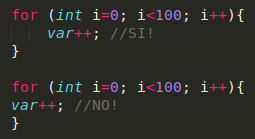
\includegraphics{indentazione1.png}
		\caption{Indentazione 1}
	\end{figure}
~\newline	
	\textbf{Indentazione 2:} È vietato l'uso di tabulazioni che possono non essere uniformi tra diversi editor o IDE. Al loro posto vanno usati gli opportuni spazi. ~\newline 
	~\newline \textbf{Indentazione 3:} Il codice che fa parte di un blocco deve essere innestato allo stesso livello di quel blocco. \newline
	\textbf{Esempio}:
	\begin{figure}[!htbp]
		\centering
		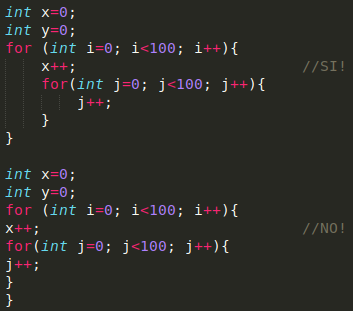
\includegraphics[scale=0.7]{indentazione3.png}
		\caption{Indentazione 3}
	\end{figure}
~\newline	
	\textbf{Parentesizzazione 1:} I blocchi di codice sono sempre racchiusi fra parentesi graffe.\newline 
	\textbf{Eccezione:} se il blocco è composto da un'unica istruzione le parentesi possono essere omesse.\newline
	~\newline
	\textbf{Parentesizzazione 2:} Le parentesi graffe iniziano sempre nella stessa linea del codice. \newline
	~\newline
	\textbf{Nomenclatura:} Classi, metodi e variabili devono avere un nome univoco e quanto più descrittivo possibile. Inoltre, devono rispettare le buone norme di scrittura in modo da distinguere immediatamente se si tratta di un nome di una classe, un metodo o una variabile. Nello specifico:\newline
	\begin{itemize}
	\item \textbf{Classi:} cominciano sempre con la lettera maiuscola;
	\item \textbf{Metodi:} cominciano sempre con una lettera minuscola e se sono composti da più parole le successive iniziano con una lettera maiuscola;
	\item \textbf{Variabili:} tutte le lettere sono minuscole ed è consentito l'utilizzo del simbolo underscore "\_".\newline
	\end{itemize}
	La lingua utilizzata deve essere l'inglese.\newline
	~\newline
	\textbf{TODO:} Un commento TODO va utilizzato per descrivere codice non definitivo, migliorabile e per soluzioni a breve termine. Può essere anche usato per eventi futuri specificando accuratamente la data.\newline
	\textbf{Esempio:}\newline
	\begin{figure}[!htbp]
		\centering
		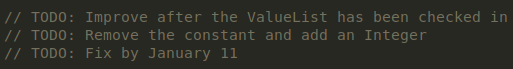
\includegraphics{todo.png}
		\caption{Esempi di TODO}
	\end{figure}
	~\newline
	\textbf{Visibilità:} Le variabili vanno dichiarate strettamente dove sono necessarie, ovvero nel blocco più interno che comprenda il loro utilizzo. Le variabili di ciclo vanno dichiarate nello statement a meno di una motivazione valida e opportunamente giustificata per non fare ciò. Le variabili globali vanno evitate in tutti i casi.\newline
	~\newline
	\textbf{Inizializzazione:} Le variabili vanno inizializzate il prima possibile, nel migliore dei casi subito dopo la loro dichiarazione. \newline
	~\newline
	\textbf{Lunghezza metodi e codice:} È da evitare una lunghezza eccessiva sia nei metodi che nelle righe di codice. Nel primo caso una giusta suddivisione rende più mantenibili i vari metodi e più chiaro il loro scopo, nel secondo rende il codice più scorrevole. \newline
	
	\paragraph{Angular} ~\newline ~\newline
	In questo paragrafo vengono descritte le norme tratte dalla \textbf{Angular-Style Guide} \footnote{\url{https://angular.io/guide/styleguide}}, la cui applicazione viene favorita da plugin opportunamente configurati in WebStorm\pedice.
	\newline
	~\newline
	\textbf{Rule of One:} Definire una funzionalità (come un service o un component) per file cercando di usare meno linee di codice possibile e funzioni piccole. Questo rende il codice più riutilizzabile, più facile da leggere e meno soggetto a errori.~\newline
	~\newline
	\textbf{Nomi dei file:} Utilizzare nomi consistenti e descrittivi, evitando abbreviazioni che possono generare confusione. Il pattern consigliato è \textit{feature.type.ts}.~\newline
	~\newline
	\textbf{Nomenclatura:} Classi, metodi, variabili e interfacce seguono le stesse regole usate nella sezione \textit{\underline{2.2.3.1}} per Javascript.~\newline
	~\newline
	\textbf{LIFT:} Strutturare l'applicazione secondo le seguenti regole:
	\begin{itemize}
	    \item \textbf{L}ocate: Fare in modo che la ricerca del codice sia intuitiva, facile e veloce;
	    \item \textbf{I}dentify: Nominare i file in modo che sia immediatamente chiaro il contenuto e cosa rappresenta;
	    \item \textbf{F}lat: Mantenere una folder structure più piatta possibile, creando sottocartelle quando sono presenti sette o più file;
	    \item \textbf{T}-DRY: Provare a essere DRY (Don't Repeat Yourself) senza sacrificare la leggibilità.~\newline
	\end{itemize}
	~\newline
	\textbf{Costanti:} Dichiarare delle variabili const solo se il valore non dovrà cambiare in futuro. Sono scritte con la prima lettera minuscola e ogni parola successiva alla prima con la maiuscola ma è tollerato anche tutto maiuscolo se sono variabili già esistenti.\newline
	\textbf{Esempio:}
	\begin{figure}[!htbp]
		\centering
		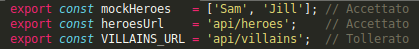
\includegraphics{constAngular.png}
		\caption{Esempio di variabili costanti}
	\end{figure}
	~\newline
	\textbf{Template e stile:} Creare file separati per template (.html) e stile (.css) quando sono più di tre righe di codice.
	\clearpage
	~\newline
	\textbf{Sequenza dei membri:} Scrivere le proprietà prima dei metodi mantenendo i membri pubblici prima di quelli privati e l'ordine alfabetico.\newline
	\textbf{Esempio:}
	\begin{figure}[!htbp]
		\centering
		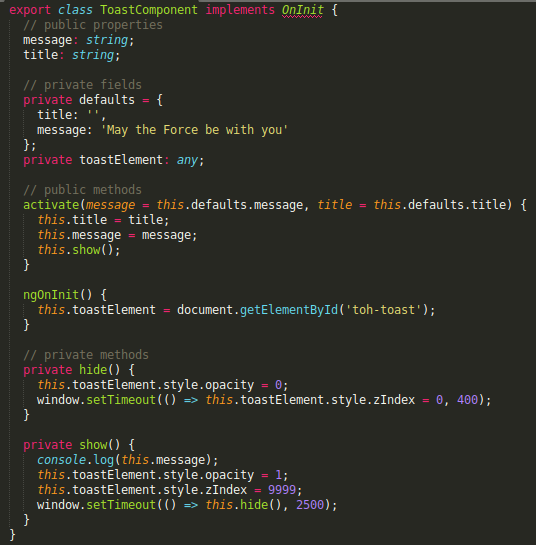
\includegraphics{sequenzaAngular.png}
		\caption{Esempio di codice ordinato correttamente}
	\end{figure}
	\clearpage
	~\newline
	\textbf{Struttura delle cartelle:} Creare una struttura di folders chiara e lineare con nomi che riflettano le caratteristiche delle feature che contengono, senza che siano ripetitivi o ridondanti. Questo aiuta a migliorare l'organizzazione in generale e la localizzazione del codice
	\paragraph{Node.js} ~\newline ~\newline
	Nonostante Node.js sia un open source server environment ci sono alcune convenzioni, tratte dalla \textbf{Node.js Style Guide}\footnote{\url{https://github.com/felixge/node-style-guide}}, da rispettare e sono le seguenti:
	\newline
	~\newline
	\textbf{Quotes:} Usare single quotes ('') invece dei double quotes ("") a meno che non si stia scrivendo un file JSON.
	\newline
	~\newline
	\textbf{Variabili:} Dichiarare una variabile per dichiarazione \textit{var}. Le variabili costanti vanno scritte in lettere maiuscole.
	\newline
	~\newline
	\textbf{Operatore di uguaglianza:} Usare sempre il triplo operatore di uguaglianza "===" per assicurarsi che i confronti si comportino sempre secondo le aspettative.
	\newline
	~\newline
	\textbf{Funzioni:} Scrivere funzioni brevi che, se necessario, ritornino un valore il prima possibile per evitare troppo annidamento.\newline
	\textbf{Esempio:}\newline
	\begin{figure}[!htbp]
		\centering
		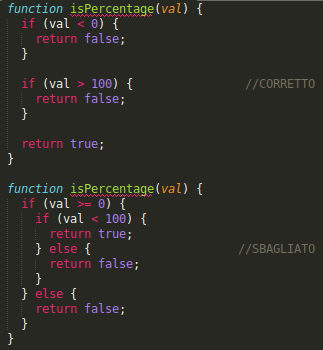
\includegraphics[scale=0.5]{funzioneNodejs.png}
		\caption{Esempio di funzione scritta correttamente}
	\end{figure}
	~\newline
	\paragraph{JSON}~\newline ~\newline
	In questo paragrafo vengono descritte le norme tratte dalla \textbf{Google JSON Style Guide}\footnote{\url{https://google.github.io/styleguide/jsoncstyleguide.xml}}, la cui applicazione viene favorita da plugin opportunamente configurati in WebStorm\pedice. ~\newline ~\newline
	\textbf{Commenti:} Non utilizzare commenti nei file JSON (in Figura \ref{json1} e Figura \ref{json2} vengono usati solo per chiarezza e solo in quanto esempi esplicativi).~\newline ~\newline
	\textbf{Quotes:} Usare sempre i double quotes ("") per i nomi  e i valori di tipo stringa delle proprietà, per gli altri valori usare i single quotes ('').~\newline ~\newline
	\textbf{Struttura dei dati:}  i dati non dovrebbero essere arbitrariamente raggruppati per convenienza~\newline
	\textbf{Eccezione:} in caso di collezioni di proprietà che rappresentano una singola struttura, è possibile tenere una gerarchia strutturata se ha senso semantico~\newline ~\newline
	\textbf{Esempio:}~\newline
	\begin{figure}[!htbp]
		\centering
		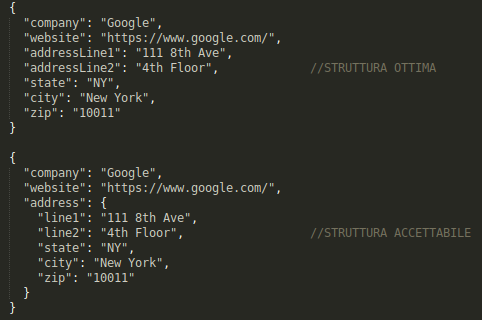
\includegraphics[scale=0.8]{datiJson.png}
		\caption{Esempio di dati in un file JSON}
		\label{json1}
	\end{figure}
	~\newline
	\textbf{Nomenclatura:} Scegliere nomi significativi per le proprietà, scrivendo la prima lettera della prima parola minuscola e per ogni parola successiva la maiuscola; usare nomi plurali solo per gli Array.~\newline ~\newline
	\textbf{Valori delle proprietà:} I valori possono essere booleani, numeri, stringhe, oggetti, array o null, cercando di evitare quest'ultimi; i tipi enum vanno rappresentati come stringhe.~\newline
	\textbf{Casi particolari:} Le date vanno formattate secondo l'RFC3339\footnote{\url{https://www.ietf.org/rfc/rfc3339.txt}}, il tempo va formattato secondo l'ISO 8601 e la latitudine e longitudine vanno rappresentate secondo l'ISO 6709.~\newline
	\begin{figure}[!htbp]
		\centering
		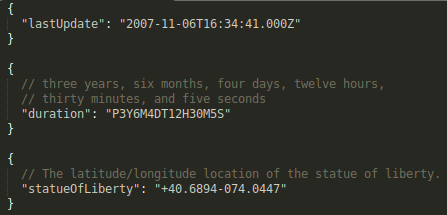
\includegraphics{casiParticolariJson.png}
		\caption{Esempio di casi particolari in un file JSON}
		\label{json2}
	\end{figure}
	~\newline
	